\documentclass[12pt,a4paper]{article}
\usepackage{rmpackages}																% usual packages
\usepackage{rmtemplate}																% graphic charter
%\usepackage{rmexocptce}																% for DS with cptce eval

%\cfoot{} 													% if no page number is needed
\renewcommand\arraystretch{1.5}		% stretch table line height

\newcounter{counterexo}
\setcounter{counterexo}{0}
\newcommand{\exo}[1]{\refstepcounter{counterexo}\subsection*{Exercice \thecounterexo{} -- #1}}

\begin{document}

\vspace*{-2.5\baselineskip}

\begin{header}
Chapitre 6 -- Décrire un mouvement
\end{header}

\section{Système, référentiel et trajectoire}

\subsection{Système}

En mécanique, le \textbf{système} est l'objet dont on étudie le mouvement.
Pour simplifier, au lycée, on modélise le système par \textbf{un point}.

\subsection{Référentiel}
\label{sec:referentiel}

On décrit toujours le mouvement d'un système par rapport à un objet de référence : c'est le \textbf{référentiel}.
Un référentiel est formé d'un \textbf{repère} dans lequel sont repérées les positions du système et d'une \textbf{horloge} pour mesurer le temps. 

\begin{multicols}{2}
\begin{center}
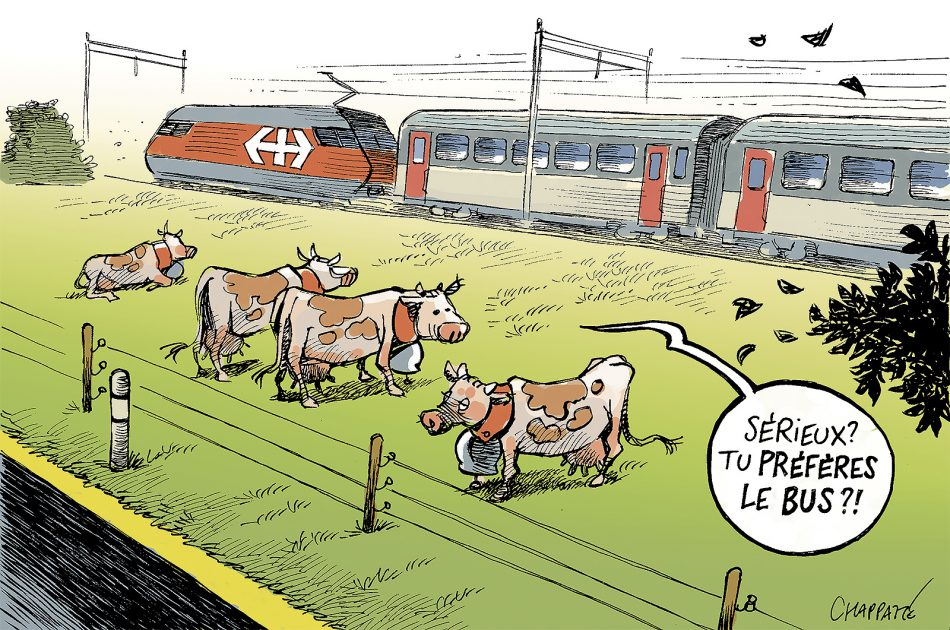
\includegraphics[trim = 60pt 0pt 10pt 0pt, clip, width=\linewidth]{images/train_cow.jpg}
% https://www.chappatte.com/images/les-bus-concurrencent-le-train/
\end{center}

\begin{em}
\textit{Cocher les propositions où le système est en mouvement par rapport au référentiel indiqué.}
\begin{itemize}
\item[$\square$] une vache par rapport au sol ;
\item[$\square$] une vache par rapport au train ;
\item[$\square$] un voyageur assis par rapport au sol ;
\item[$\square$] un voyageur assis par rapport au train ;
\item[$\square$] un voyageur allant au wagon bar par rapport au sol ;
\item[$\square$] un voyageur allant au wagon bar par rapport au train.
\end{itemize}
\end{em}
\end{multicols}

\textbf{Le mouvement d'un système dépend du référentiel choisi !}
Souvent, un référentiel est plus adapté à l'étude du mouvement d'un système.
Dans ce référentiel privilégié, le mouvement du système est \textbf{simple}.

\begin{center}
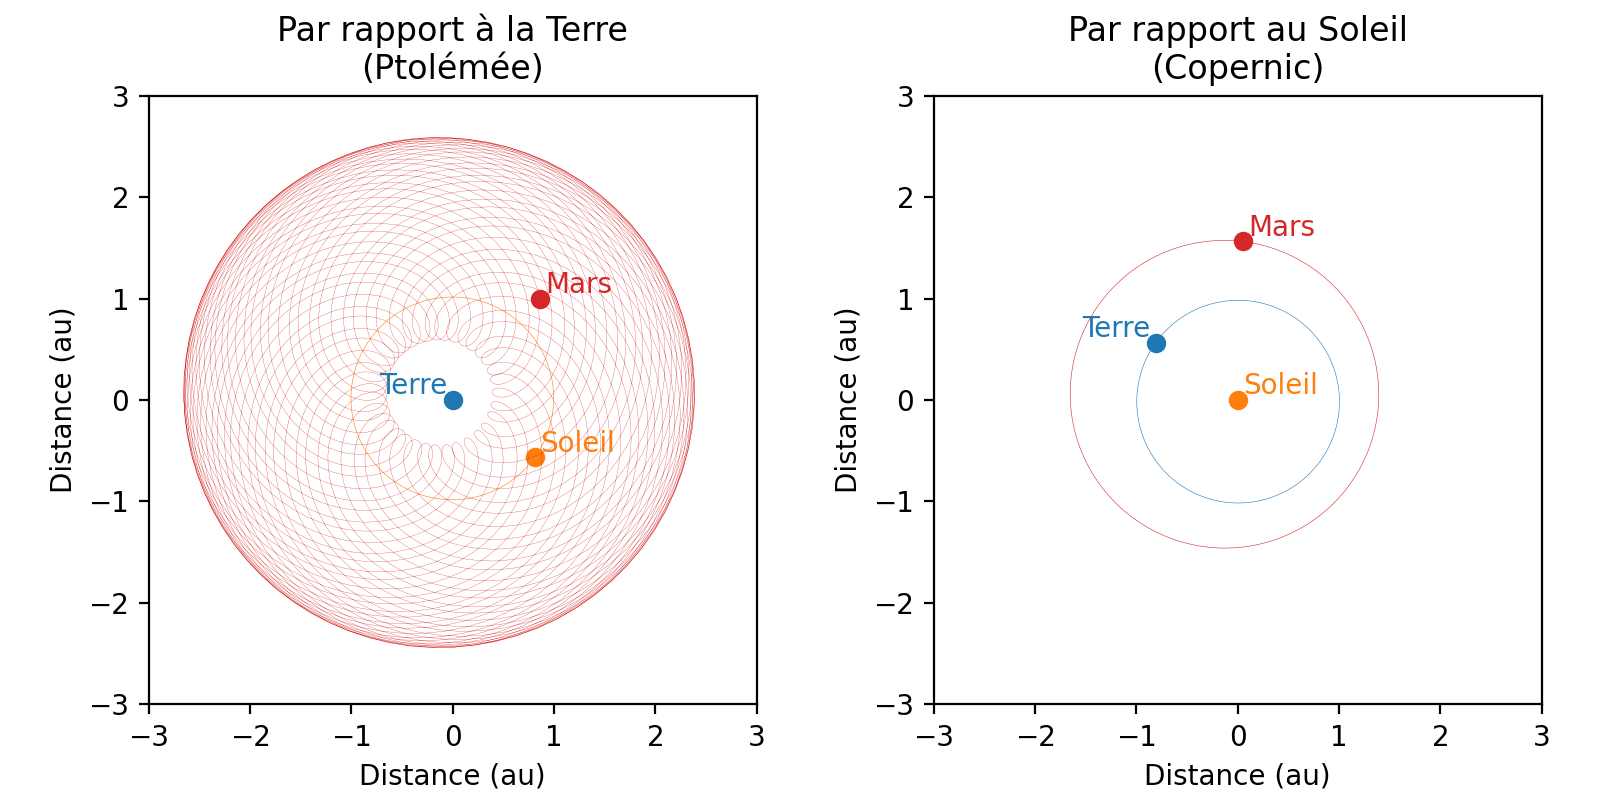
\includegraphics[scale=0.75]{images/retrograde_motion.png}
\end{center}

\subsection{Trajectoire}

La \textbf{trajectoire} d'un système est l'ensemble de ses positions successives au cours du temps.
Elle \textbf{dépend du référentiel}.

\begin{multicols}{3}
\begin{center}
\textcolor{bleu_f}{Mouvement \textbf{rectiligne}}

\begin{tikzpicture}
\foreach \x in {0,0.6666,...,4} {
  \draw (\x,\x) node [color=bleu_f] {$\bullet$};
}
\draw [color=bleu_f, dashed] plot [domain=0:4] (\x, \x);
\end{tikzpicture}

\textcolor{green_f}{Mouvement \textbf{circulaire}}

\begin{tikzpicture}
\foreach \x in {0,0.16666,...,1.6667} {
  \draw (180*\x-20:2) node [color=green_f] {$\bullet$};
}
\draw [color=green_f, dashed] plot [domain=0:1.6667, smooth] (180*\x-20:2);
\end{tikzpicture}

\textcolor{red_f}{Mouvement \textbf{curviligne}}

\begin{tikzpicture}
\foreach \x in {-2,-1.6667,...,2} {
  \draw (\x,-\x*\x) node [color=red_f] {$\bullet$};
}
\draw [color=red_f, dashed] plot [domain=-2:2] (\x, -\x*\x);
\end{tikzpicture}
\end{center}
\end{multicols}

\begin{em}
Caractériser le mouvement de chaque système dans les trois cas suivants.
\begin{itemize}
\item[•] La Lune, par rapport à la Terre :
\item[•] Usain Bolt courant un 100 mètres, par rapport à la piste :
\item[•] Un avion qui décolle, par rapport à la piste :
\end{itemize}
\end{em}

\section{Vitesse et vecteur vitesse}

\subsection{Vitesse moyenne}

\vfill\hfill
\begin{tikzpicture}
\coordinate (A) at (0,3);
\coordinate (B) at (6,0);
\draw (A) node {$\times$} node [below left] {$O$};
\draw (B) node {$\times$} node [below right] {$M$};
\draw [dashed] (A) -- (B) node [midway, above] {$d$};
\end{tikzpicture}
\vfill

La vitesse moyenne ne dépend pas de la trajectoire du système.

\begin{multicols}{2}
\begin{center}
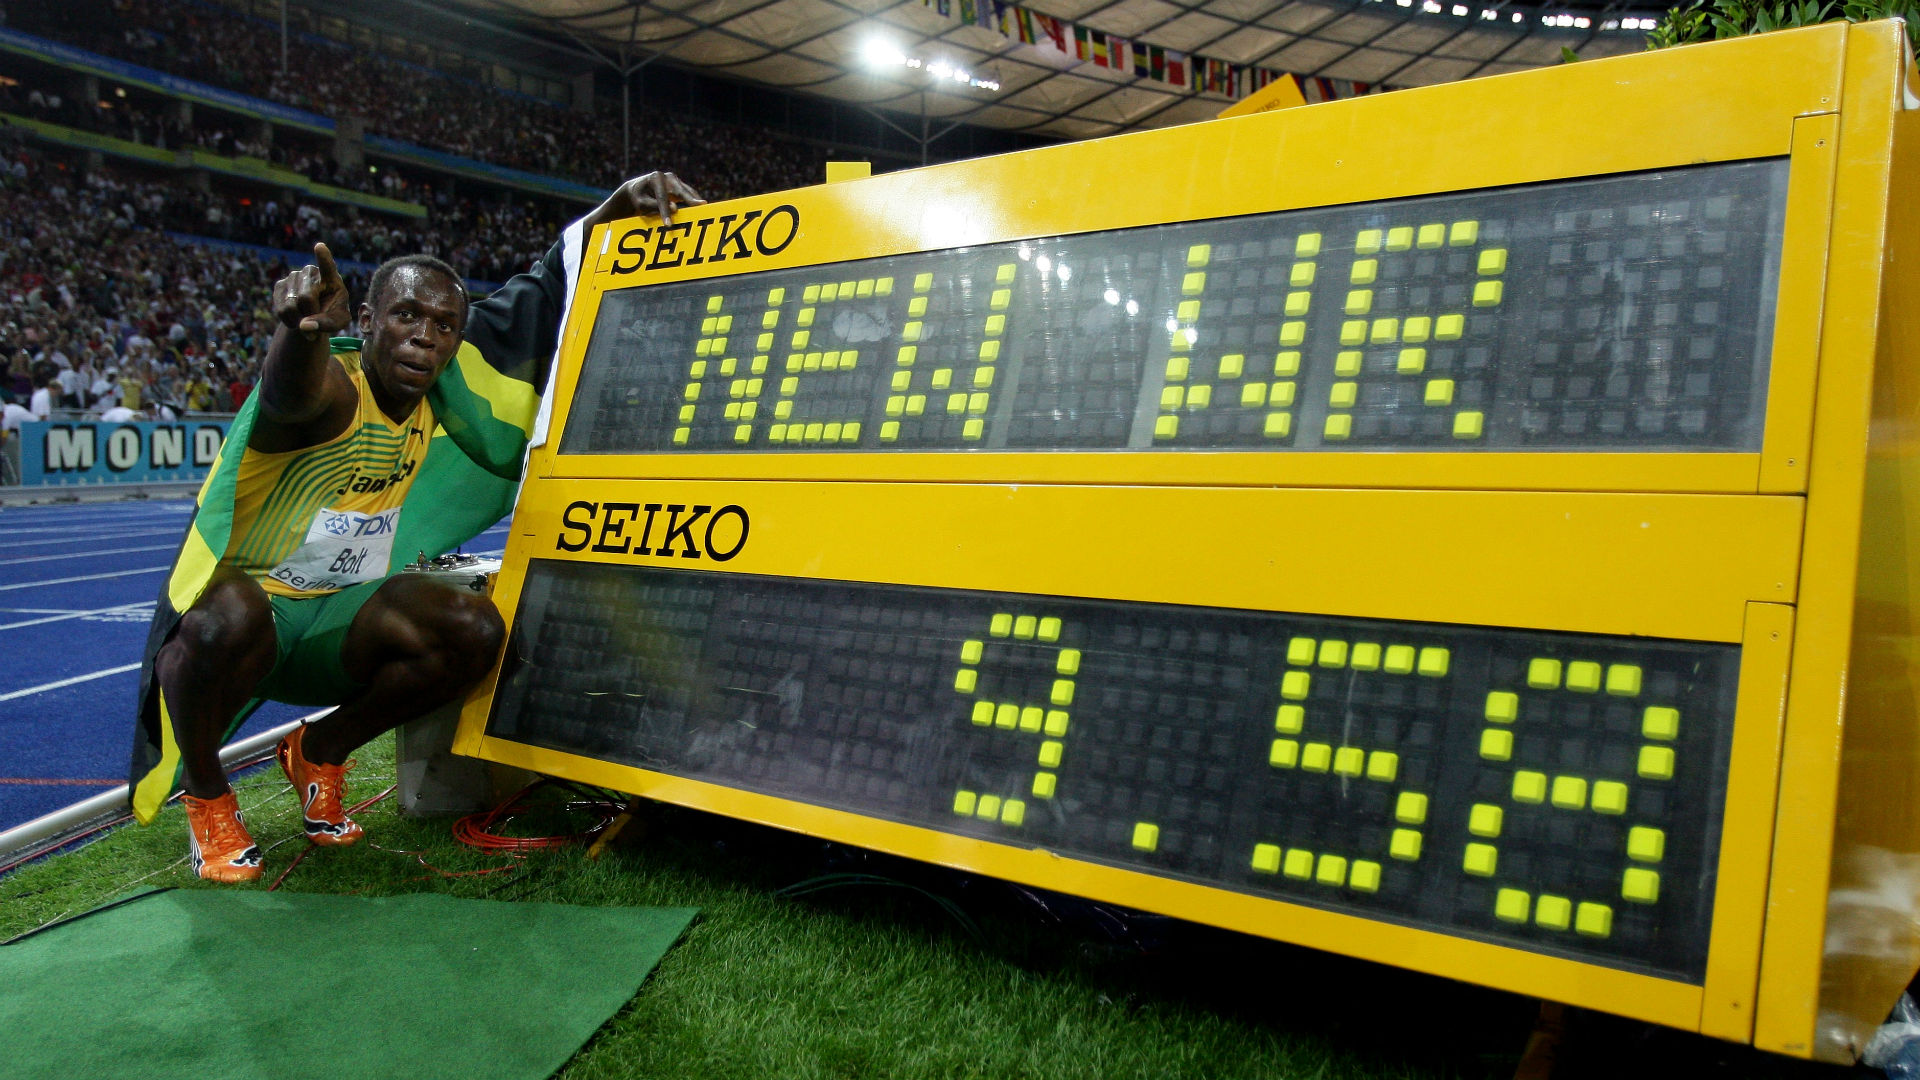
\includegraphics[width=\linewidth]{images/usain_bolt_wr.jpg}
\end{center}

\begin{em}
Le 16 août 2009, en final des championnats du monde d'athlétisme, Usain Bolt établissait un nouveau record du monde du 100 mètres avec un temps de 9{,}58 secondes.
Calculer sa vitesse moyenne pendant la course.
\end{em}
\end{multicols}

On dit que le mouvement est \textbf{uniforme} quand \textbf{la valeur de la vitesse reste constante}.
Sinon, on dit que le mouvement est \textbf{non uniforme} (accéléré ou décéléré).

\subsection{Le vecteur vitesse}

\begin{center}

\begin{tikzpicture}
\def\length{13.5};
\def\width{3}
\coordinate (A) at (-\width/2,0);
\coordinate (B) at (\length,\width);
\coordinate (C) at (-\width/2,\width/2);
\coordinate (D) at(\length,\width/2);
\draw [line width=2, color=gray_c] (A) rectangle (B);
\draw [line width=2, color=gray_c] (C) -- (D);
\draw [line width=5, color=gray_c] (0,0) -- (0, \width);

\def\squarewidth{\width/14}

\draw [line width=2, color=gray_c] (\length-\squarewidth, 0) rectangle (\length+\squarewidth, \width);
\foreach \n in {0, 1, ..., 6} {
  \def\y{\n*\width/7}
  \fill [color=gray_f] (\length-1*\squarewidth, \y) rectangle (\length-0*\squarewidth, \y+\squarewidth);
  \fill [color=gray_f] (\length-0*\squarewidth, \y+\squarewidth) rectangle (\length+1*\squarewidth, \y+2*\squarewidth);
}

\draw (C) + (-.5,0) node [rotate=-90, color=gray_f] {\large\textbf{DÉPART}};
\draw (D) + (\squarewidth+.5,0) node [rotate=-90, color=gray_f] {\large\textbf{ARRIVÉE}};
\draw (-\width/4, 3*\width/4) node [rotate=-90, color=gray_f] {\Large\textbf{1}};
\draw (-\width/4, \width/4) node [rotate=-90, color=gray_f] {\Large\textbf{2}};

\def\d{\length*0.5}

\coordinate (M) at (\d/2, 3*\width/4);
\draw (M) node {$\times$};
\draw (M) node [above left] {$M$};
\node[inner sep=0pt, opacity=.25] (turtle) at (M) {
\includegraphics[scale=.04]{images/turtle.png}};

\coordinate (N) at (\d, \width/4);
\draw (N) node {$\times$};
\draw (N) node [above left] {$N$};
\node[inner sep=0pt, opacity=.25] (panpan) at (N) {
\includegraphics[scale=.07]{images/panpan.jpg}};
\end{tikzpicture}
\end{center}

\paragraph{Caractéristiques du vecteur vitesse :}
\begin{itemize}
\item[\phantom{•}]
\item[\phantom{•}]
\item[\phantom{•}]
\item[\phantom{•}]
\item[\phantom{•}]
\item[\phantom{•}]
\item[\phantom{•}]
\end{itemize}

\begin{em}
On s'intéresse au mouvement d'une grenouille par rapport au sol alors qu'elle fait un bond.
Représenter le vecteur vitesse pour les positions successives de la grenouille.
\end{em}

\begin{center}
\begin{tikzpicture}
\foreach \t in {0,1,...,6} {
  \coordinate (M) at (10*1.5*\t/6, 10*(-10/2*\t*\t/6/6 + 10/2*\t/6);
  \node[inner sep=0pt, opacity=.25] (frog) at (M) {
\includegraphics[scale=.1]{images/frog.png}};
  \draw (M) node {$\times$};
  \draw (M) node [below left] {$M_\t$};
}
\draw (7.5,2*\baselineskip) node [color=gray_f] {Les positions de la grenouille sont relevées toutes les \unit{0{,}167}{s}.};
\draw (7.5,\baselineskip) node [color=gray_f] {Le schéma est à l'échelle 1/10 : \unit{1}{cm} sur le schéma = \unit{10}{cm} en vrai.};
\draw (7.5,0) node [color=gray_f] {Échelle pour les vecteurs vitesse : $\unit{1}{cm} \leftrightarrow \unit{1}{m/s}$.};
\end{tikzpicture}
\end{center}

\section{Applications}

\exo{Choisir un référentiel}

En reprenant l'illustration de la section \ref{sec:referentiel} et pour chacun des systèmes suivants, indiquer le référentiel par rapport auquel le mouvement du système est le plus simple.
\begin{center}
\begin{tabular}{|l|c|c|c|c|}
\hline
\textbf{Système}		& une vache	& un voyageur assis & un voyageur allant au wagon bar & le train \\
\hline
\textbf{Référentiel}	& & & & \\
\hline
\end{tabular}
\end{center}

\section{Exercices}

\begin{multicols}{2}
\begin{itemize}
\item[•] QCM bilan page 157 (sauf question 9) ;
\item[•] 4 page 160 ;
\item[•] 6 page 160 ;
\item[•] 9 page 161 ;
\item[•] 20 page 162 ;
\item[•] 22 page 163 ;
\item[•] 19 page 162 ;
\item[•] 21 page 162.
\end{itemize}
\end{multicols}

\end{document}

\begin{tikzpicture}
\coordinate (A) at (0,0);
\coordinate (B) at (6,2);
\draw (A) node {$\times$};
\draw (A) node [below] {$M$};
\node[inner sep=0pt, opacity=.25] (panpan) at (A) {
\includegraphics[scale=.07]{images/panpan.jpg}};
\draw (B) node {$\times$};
\draw (B) node [below] {$M'$};
\node[inner sep=0pt, opacity=.25] (panpan) at (B) {
\includegraphics[scale=.07]{images/panpan.jpg}};

\coordinate (A) at (9,0);
\coordinate (B) at (15,2);
\draw (A) node {$\times$};
\draw (A) node [below] {$M$};
\node[inner sep=0pt, opacity=.25] (turtle) at (A) {
\includegraphics[scale=.04]{images/turtle.png}};
\draw (B) node {$\times$};
\draw (B) node [below] {$M'$};
\node[inner sep=0pt, opacity=.25] (turtle) at (B) {
\includegraphics[scale=.04]{images/turtle.png}};
\end{tikzpicture}